\chapter*{Copies of publications - Publikacijų kopijos}
\label{cha:publicationscopies} 
\addcontentsline{toc}{chapter}{\MakeUppercase{Copies of publications - Publikacijų kopijos}}
%kai disertacija parengta mokslinių straipsnių rinkinio pagrindu)
%Used, when you do not write a regular dissertation, you may need to include full papers in the dissertation
% \parammarks{Copies of publications}

%\index{publications} 

%  VU Leidykla paprasys prideti titulini lapa pries kiekviena publikacija. Kaip tai padaryti yra jusu pasirinkimas, bet galetu atrodyti taip:

\vspace*{15mm}

\begin{center}

{\huge 1st publication}
\vspace{10mm}

{\Large \bf Modeling the uptake of fluorescent molecules into 3D cellular spheroids}

\vspace{5mm}
\textbf{R. Astrauskas}, F. Ivanauskas, G. Jarockytė, V. Karabanovas, and R. Rotomskis

\vspace{5mm}
\textit{Nonlinear Analysis: Modelling and Control}, 24(5): 838--852, 2019


\vspace{3mm}
DOI: 10.15388/NA.2019.5.9

\end{center}

\newpage
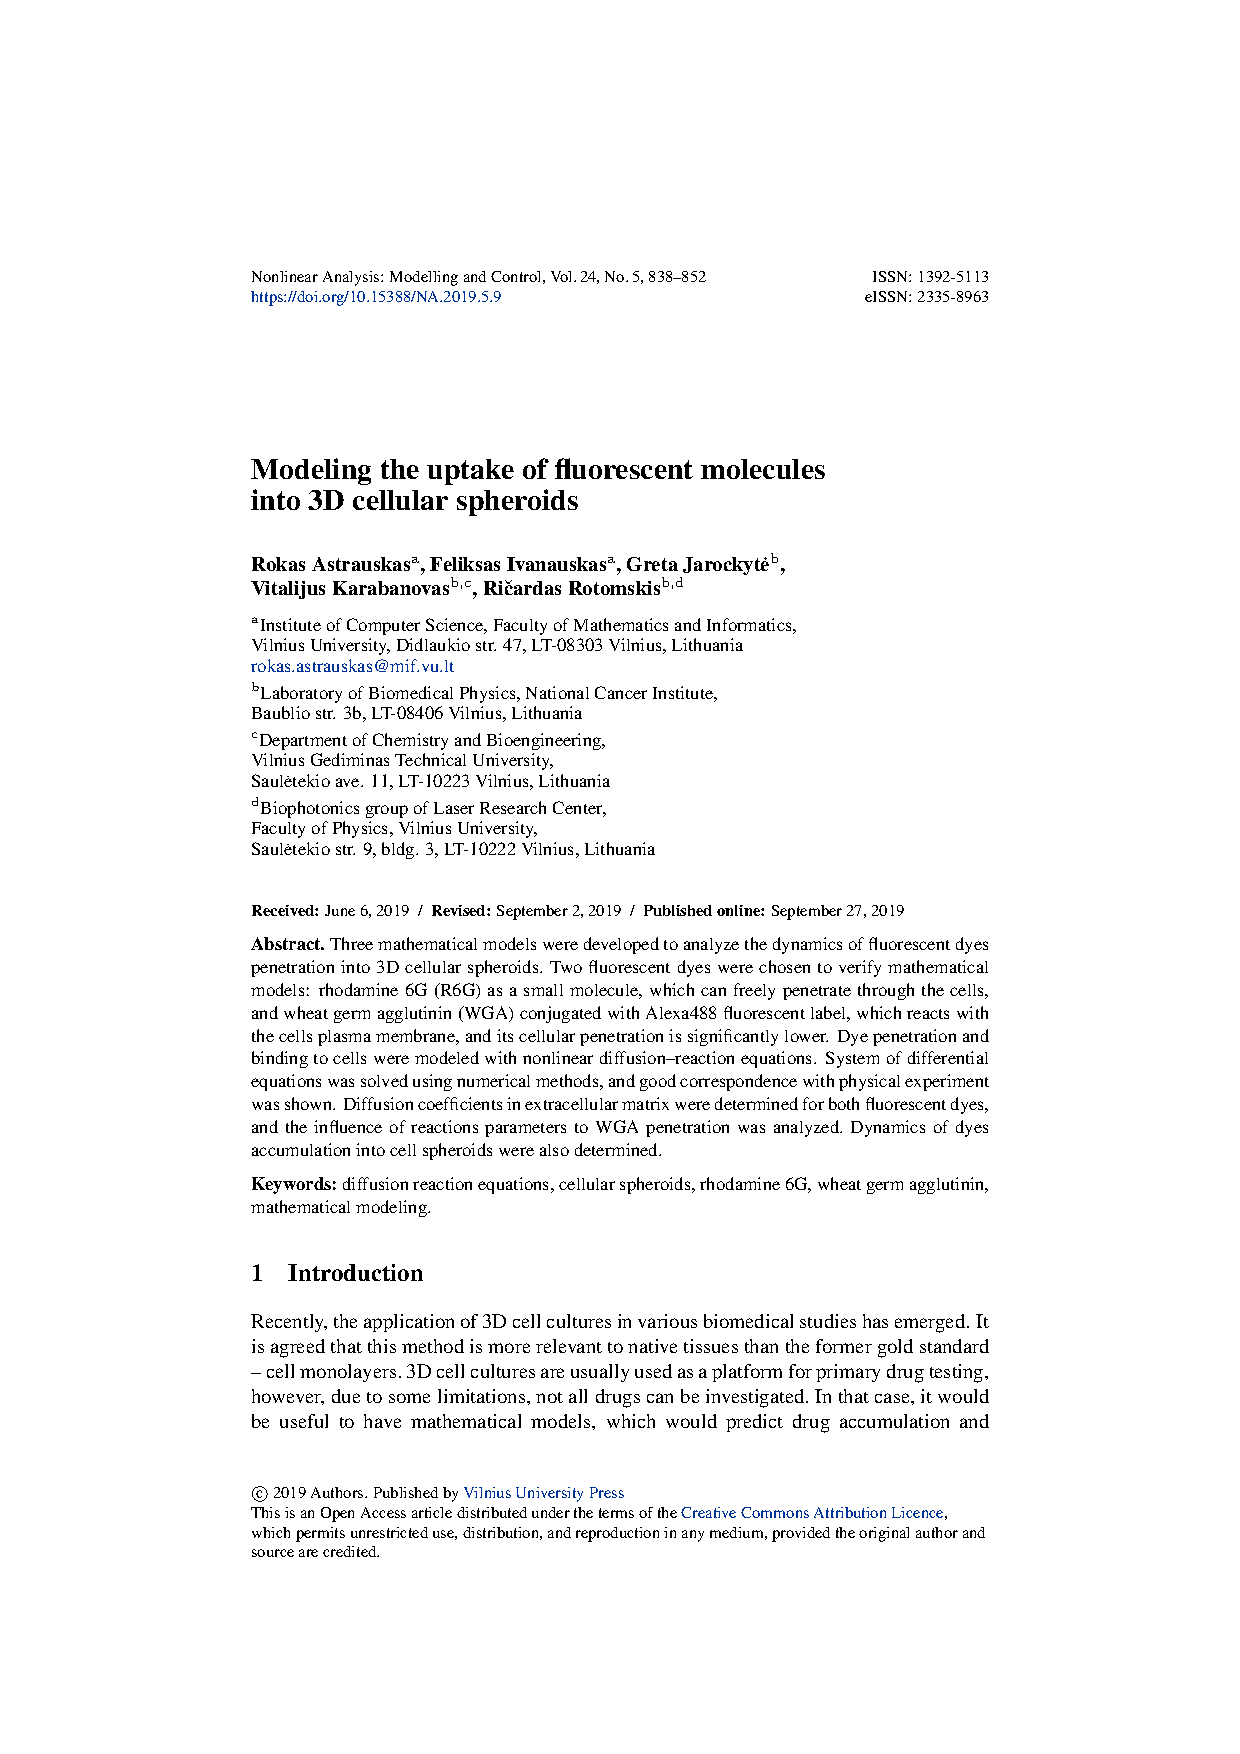
\includepdf[scale=1., pages=-]{publications/Astrauskas2019spheroids.pdf}